%LaTeX SAMPLE FILE FOR PAPERS OF CDAM

% LaTeX 2e
\documentclass[12pt]{article}

\usepackage{graphicx}
\usepackage{epsfig}
\usepackage{cite}
\usepackage{amsmath,amssymb,amsfonts,amsthm}
\usepackage[boxed]{algorithm2e}
\usepackage{caption}
\usepackage{wrapfig}
\usepackage{upgreek}
\usepackage{adjustbox}
\usepackage{pbox}
\usepackage{index}
\usepackage{color}
\usepackage{makecell}
\usepackage{multirow}
\usepackage{bbm}
\usepackage{lastpage}
\usepackage{longtable}
\usepackage{changepage}

% LaTeX 2.09
%\documentstyle[12pt]{article}

%%%%%%%%%%%%%%%%%%%%%%%%%%%% paper layout %%%%%%%%%%%%%%%%%%%%%%%%%%%%%%
\hoffset=-1in
\voffset=-1in
% Please, don't change this layout
\parindent=6mm
\topskip=0mm
\topmargin=30mm
\oddsidemargin=27.5mm
\evensidemargin=27.5mm
\textwidth=155mm
\textheight=237mm
\headheight=0pt
\headsep=0pt
\footskip=2\baselineskip
\addtolength{\textheight}{-\footskip}

\providecommand{\keywords}[1]
{
\vspace{2mm}\hspace{20pt}\textbf{\textit{Keywords:}} #1
}

\providecommand{\abskeyw}[2]
{
\begin{small}
\begin{adjustwidth}{10mm}{10mm}
\vspace{1mm}\hspace{20pt}#1

\keywords{#2}
\end{adjustwidth}
\end{small}
}

\begin{document}

%%% Title section
\begin{center}
{\Large\bf SHORT-TERM FORECASTING AND NOWCASTING OF GDP GROWTH RATES IN THE REPUBLIC OF BELARUS USING MIXED FREQUENCY VECTOR AUTOREGRESSIVE MODELS}\\\vspace{2mm} {\sc T.A.
Bout$^1$, V.I. Malugin$^2$}\\\vspace{2mm}
{\it Belarusian State University\\
Minsk, BELARUS\\} e-mail: {\tt $^1$bout.timofey@gmail.com,
$^2$Malugin@bsu.by}

\abskeyw{The article presents the results of constructing vector autoregressive models based on mixed frequency data, designed for short-term forecasting and science-casting of real GDP growth rates in the Republic of Belarus based on economic indicators available with a monthly frequency of observation. A comparative analysis of the accuracy of short-term forecasts and nowcasts is carried out based on the constructed models based on mixed and aggregated data.}{mixed frequency data, short term forecasting and nowcasting, MF-VAR model, real GDP growth rates forecasting, macroeconomic indicators.}
\end{center}

\section{The relevance of the problem and the purpose of the study}

The first official estimate of the real gross domestic product (GDP) is formed by the National Statistical Committee of the Republic of Belarus (NSC RB) on a quarterly frequency on the 90th day after the reporting period, i.e. with a delay of one quarter. At the same time, statistics on industry indicators and price indices are generated on a monthly basis and published in the month following the reporting month – two months before the end of the current quarter. In this regard, the task of forecasting real GDP for the past, current and near future quarters based on available monthly data becomes urgent. This task of assessing the current state of the modeled process is known as the nowcasting task \cite{1}. Obviously, the accuracy of forecasts for subsequent periods depends on the assessment of the current state.

The purpose of the study is to build vector autoregression models based on mixed data (\textit{Mixed Frequency Vector Autoregression} -- MF–VAR) \cite{2}, designed for short-term forecasting one quarter ahead and tracking real GDP growth rates based on economic indicators available with a monthly frequency of observation; a comparative analysis of the accuracy of forecasts of the constructed models for mixed and aggregated data. The problem under consideration has been solved in various countries, including the Russian Federation \cite{4}. This task has not been considered before for the Belarusian economy.

\section{Description of the models}

When building the models, the following tasks were solved: 1) pre-processing of time series (seasonal adjustment, logarithmization, reduction to a stationary form by reducing to growth rates); 2) selection of optimal model specifications; 3) evaluation, analysis of statistical adequacy and assessment of forecast accuracy.

The following time series of economic indicators provided by the NSC of the Republic of Belarus were used to conduct the research:
\begin{itemize}
	\item PC\_LRGDP -- growth rates in logarithms of the real quarterly GDP of Belarus by sources of income use in average annual prices in 2018, million rubles, YoY (in \%);
	\item PC\_LRPP\_M\_SA -- the growth rate in logarithms of industrial production in average annual prices in 2018, MoM (in \%);
	\item PC\_LRRET\_M\_SA -- the growth rate in logarithms of retail turnover in average annual prices in 1995, MoM (in \%);
	\item PC\_LRINV\_M\_SA -- growth rates in logarithms of the volume of investments in fixed assets at average annual prices in 2018, MoM (in \%);
	\item PC\_LRAGRO\_M\_SA -- the growth rate in logarithms of the volume of agriculture in the average annual prices of 2018, MoM (in \%);
	\item PC\_LBI\_BLD\_M\_SA -- the growth rate in logarithms of the basic index of the volume of construction and installation works (January 2018 = 1), MoM (in \%);
	\item PC\_LBI\_RRDH\_M\_SA -- the growth rate in logarithms of the basic index of the volume of monetary incomes of the population (January 2018 = 1), MoM (in \%);
	\item CESI\_M\_SA is a composite economic sentiment index \cite{5}.
\end{itemize}
The \_SA symbols indicate a seasonally adjusted time series using the TRA-MO/SEATS method.

A constant and an impulse dummy variable dum2022q2 were also added to the model to account for the structural change in the second quarter of 2022. The MF-VAR($p$) model, estimated using the least squares method, consists of $22$ equations (one for the target quarterly indicator and three equations for each monthly indicator corresponding to 1, 2 and 3 months in the block). Thus, the number of estimated parameters is $22(2+22 p)$, where $p$ corresponds to the number of lags for the variables.

\section{Comparative analysis of forecast accuracy}

The accuracy of one-step forecasts for one quarter ahead for models based on mixed data (MF-VAR) and aggregated data (VAR) was assessed using retrospective forecasts during the model evaluation period, as well as on the basis of non-selective one-step forecasts using the "expanding window" algorithm. According to this algorithm, forecasts for the period from the third quarter of 2022 to the fourth quarter of 2024 were made with sequential progress for one quarter. Thus, 10 quarterly forecasts were obtained for the predicted variables, on the basis of which the following forecast accuracy characteristics were calculated: RMSE (Root Mean Squared Error) and MAE (Mean Absolute Error). The values of these characteristics for the target are shown in Table 1 for the MF-VAR and VAR models.

All the models presented in Table 1 have an optimal specification in terms of metrics. The VAR and MF-VAR models include all the described macroeconomic indicators, regardless of their significance. The VAR$^*$ model includes only the PC\_LRPP\_M\_SA variable as significant and best in terms of metrics; the MF-VAR$^*$ model includes the PC\_LRPP\_M\_SA, PC\_LRRET\_M\_SA, and CESI\_M\_SA variables as best in terms of metrics.
	
	\begin{table}[h!]
		\centering
		\caption{Accuracy Indicators for Forecasting Annual GDP Growth Rates of RB}
		\label{tab:forecast_accuracy}
		\begin{tabular}{|>{\centering\arraybackslash}p{5cm}|>{\centering\arraybackslash}p{4cm}|>{\centering\arraybackslash}p{4cm}|}
			\hline
			\textbf{Model} & \textbf{RMSE} & \textbf{MAE} \\ \hline
			\multicolumn{3}{|c|}{Forecasting Period 2022Q3 -- 2024Q4 (Retrospective Forecasts)} \\ \hline
			VAR(5)        & 1.542778      & 1.192851      \\ \hline
			VAR*(5)       & 3.095332      & 2.563846      \\ \hline
			MF-VAR(2)     & 1.335281      & 1.064489      \\ \hline
			MF-VAR*(5)    & \textbf{0.5603*} & \textbf{0.3970*} \\ \hline
			\multicolumn{3}{|c|}{Forecasting Period 2022Q3 -- 2024Q4 (Expanding Window with a Step of 1)} \\ \hline
			VAR(1)        & 2.495408      & 1.877692      \\ \hline
			VAR*(2)       & 2.112804      & 1.424611      \\ \hline
			MFVAR(1)      & 3.106951      & 2.375936      \\ \hline
			MFVAR*(2)     & \textbf{1.8467*} & \textbf{1.2564*} \\ \hline
		\end{tabular}
	\end{table}
	
Based on the results of a comparative analysis of forecast accuracy metrics (Table 1), the MF-VAR* model has the best forecast accuracy indicators. 

In Figure 1 we see a graph of one-step out-of-sample forecasts using the expanding window algorithm.

\begin{figure}[htbp]
	\centering
	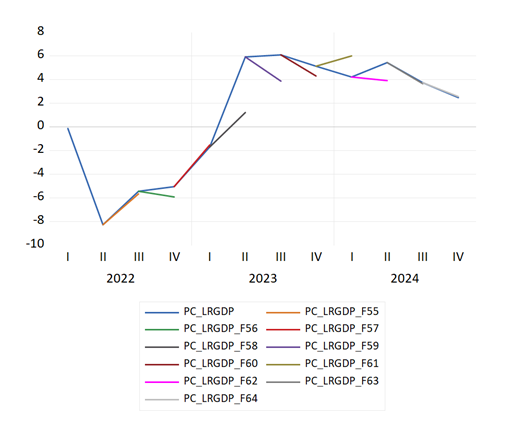
\includegraphics[width=0.5\textwidth]{graph01}
	\caption{Forecast of non-selective values of real GDP growth in Belarus based on the MFVAR model for the best combination of variables}
	\label{fig:graph01}
\end{figure}

\section{Conclusion}

As a result of the study, it was found that the best combination of variables for predicting GDP growth in the Republic of Belarus in terms of metrics is PC\_LRPP\_M\_SA, PC\_LRRET\_M\_SA, CESI\_M\_SA, with the number of lags $p=2$. The result also corresponds to the economic meaning of the constructed model. Indeed, industrial production (PC\_LRPP\_M\_SA) and retail trade (PC\_LRRET\_M\_SA) are approximations of those components that account for the largest share of the total GDP of Belarus in terms of added value; and the CESI indicator can be interpreted as the average expected value of GDP over a certain period.

Based on the results obtained, the following conclusions can be drawn:
\begin{enumerate}
	\item [1)] the MF-VAR model based on mixed frequency data, with the best selection of high-frequency variables, is able to make more accurate forecasts compared to the VAR model based on aggregated data in the mode of short-term forecasting and nowcasting; 
	\item [2)] nn the short term, the real GDP of the Belarusian economy is most influenced by such macroeconomic indicators as the volume of industrial production, the volume of retail trade and the CESI economic sentiment index.
\end{enumerate}

%% please make bibitems content in a style below !!!
%% papers with "free style" bibitems content will be rejected !!!

\begin{thebibliography}{10}

\bibitem{1}
BańBura M., Giannone D., Reichlin L. (2012). {Nowcasting}. \textit{The Oxford Handbook of Economic Forecasting}, pp. 193–224.

\bibitem{2}
Foroni C., Marcellio M. (2013). \textit{A survey of econometric methods for mixed frequency data}. {Working Paper} Vol. 6, Norges Bank, 45 p.

\bibitem{3}
Kharin Yu.S., Malugin V.I., Kharin A.Yu. (2003). \textit{Econometric Modeling: A Study Guide}. Minsk, BSU, 318 p. (In Russian)

\bibitem{4}

Makeeva, N.M., Stankevich I.P. (2020). {Nowcasting Elements of GDP Use in Russia}. \textit{Economic Journal of the Higher School of Economics}. Vol. 10, 25 p. (In Russian)

\bibitem{5}

Malugin V., Kruk D., Milevsky P. (2019) Economic Sentiment Index of the Belarusian Economy: Methodological, Model, and Software Tools. \textit{Banking Bulletin Journal}, Bank Research No. 16, 31 p. (In Russian)

\end{thebibliography}


\end{document}
